% Chapter 5

\chapter{LEFTy}

\label{Chapter5} % For referencing the chapter elsewhere, use \ref{Chapter5} 

LEFTy --- por sus siglas en inglés: Language Efficient Text Portray --- es el nombre designado para referirse al trabajo actual. Esta solución propuesta emplea el concepto de \textit{transfer learning} para poder permitir entrenar con gran capacidad tareas que no tienen muchos ejemplos etiquetados. Utiliza una RNN como base del modelo y las características base obtenidas fueron:

\begin{itemize}
\item \textbf{Edad.}
\item \textbf{Género.}
\item \textbf{Región de origen.}
\end{itemize}

\section{Pre-entrenamiento de modelo de lenguaje}

La fase de pre-entrenamiento en el contexto de NLP consiste en entrenar una especie de modelo de lenguaje. En el artículo original de ULMFiT \parencite{howard2018}, se utiliza un modelo estándar en donde se predice el siguiente token basado en una cadena de tokens. BERT \parencite{devlin2018bert} por otro lado utiliza un Masked Language Model (MLM) el cual consiste en predecir el 15\% de los tokens dado todo el contexto que los rodea.

\subsection{Modelo de lenguaje de Wikipedia}

El diseño base para este modelo de lenguaje es una red denominada AWD LSTM \parencite{merityRegOpt}, la cual emplea una modificación agresiva al método de regularización \textit{dropout}. En el artículo se sugiere utilizar un concepto denominado \textit{DropConnect} y difiere en \textit{dropout} en que las funciones de activación no son las que toman el valor cero, sino los pesos. También se utilizan los conceptos de usar \textit{dropout} en la capa de vectorización de palabras --- esto no aporta a la regularización pero sí disminuye el tamaño de los vectores representantes de los vectores. Se instancian los distintos tipos de \textit{dropout} con pesos asignados a cada uno. En el artículo se recomiendan usar ciertos pesos base y optimizar un hiperparámetro $r_f$ únicamente el cual le da escala a los pesos recomendados y definidos por ellos.

En el capítulo \ref{Chapter4} se explica el pre-procesamiento que se le da a los datos de \textit{Wikipedia}. Se detallará ese proceso a continuación.

Para realizar este procedimiento se utilizaron los recursos de \emph{Google Colaboratory} (Colab), los cuales ofrecen un ambiente de \textit{Notebooks} de IPython y la habilidad de ejecutar comandos de \*nix.

\begin{figure}
\centering
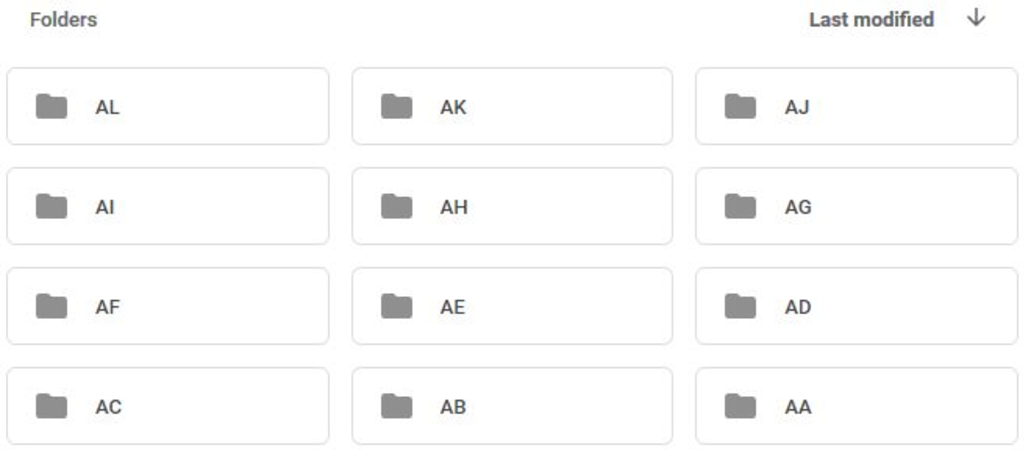
\includegraphics[scale=0.7]{Figures/wikidump.pdf}
\caption{Estructura de datos resultante al extraer un archivo de \textit{Wikipedia}.}
\label{fig:wikidump}
\end{figure}


\textbf{Obtención de datos.} El corpus de Wikipedia fue obtenido del sitio oficial (\url{https://dumps.wikimedia.org/eswiki/}). El corpus obtenido fue de noviembre 2018. Estos archivos tienen una estructura específica y la forma recomendada de extraer sus contenidos es utilizando \emph{WikiExtractor} (\url{https://github.com/attardi/wikiextractor}). Esta herramienta permite realizar una extracción que filtra por un parámetro de mínimo de longitud del artículo. Se utilizó este parámetro para filtrar todos los artículos con menos de 10,000 caracteres.

Una vez finaliza la extracción del archivo --- la cual demora una cantidad no despreciable de horas --- se procede a leer y filtrar los documentos. En el caso de este trabajo se filtraron todos los documentos después de haber acumulado 100 millones de tokens en lo seleccionado. Se conservaron 10 millones de tokens adicionales para la validación de resultados.

\begin{table}
\begin{tabular}{| l | l |}

\hline
\textbf{Cadena de caracteres} & \textbf{Resultado tokenizado} \\
\hline
Hola, buenos días. & \texttt{xxbos xxmaj hola , buenos días} \\
HOLA!!! qué bueno verte & \texttt{xxbox xxmaj hola xxrep 3 ! qué bueno verte} \\
Mis audífonos son Sennheiser & \texttt{xxbos xxmaj mis audífonos son xxunk} \\
\hline

\end{tabular}
\caption{Muestras de tokenización utilizando \textit{spaCy} y técnicas de \textit{fastai}}
\label{tab:tokens}
\end{table}

\textbf{Tokenización.} La herramienta utilizada para este proceso fue spaCy (\url{https://spacy.io/}). Esta herramienta tiene soporte para más de 34 idiomas, entre los cuales está incluído el español. Además de esta herramienta se emplean técnicas adicionales como codificar caracteres repetidos o codificar palabras en mayúsculas.

\textbf{Definición de vocabulario.} Como se puede apreciar en el cuadro \ref{tab:tokens}, unos tokens son codificados como \texttt{xxunk}, esto es debido a la limitación de palabras únicas a codificar. El vocabulario fue limitado a 30,000 tokens únicos.

\begin{figure}
\centering
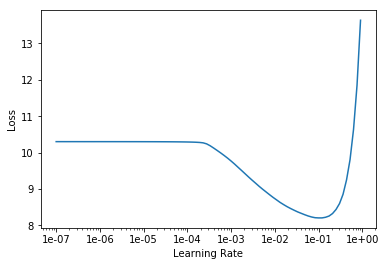
\includegraphics[scale=1]{Figures/lrfinder.png}
\caption{Ilustración de progreso de la función \texttt{lr\_find} de \textit{fast.ai}. Al momento de divergir el método deja de aumentar $\gamma$ y devuelve los resultados.}
\label{fig:lrfind}
\end{figure}

\textbf{Entrenamiento.} Luego tener los datos en el formato adecuado para entrenar el modelo se aplican las técnicas descritas en el capítulo \ref{Chapter3} sobre una red AWD LSTM. Previo a esto se encuentra un $ \gamma $ ideal y eso se hace aprovechando el método \texttt{lr\_find} (figura \ref{fig:lrfind}) de la librería de \emph{fastai} (\url{https://github.com/fastai/fastai}) que emplea el método descrito por \textcite{smith2017convergence}. Se aumenta $\gamma$ a medida que se recorren los ejemplos a entrenar. Si en algún momento diverge el aprendizaje se detiene el método y se imprime la gráfica. Se deberá querer elegir un $\gamma$ que no tenga riesgo de divergir el aprendizaje y que tampoco disminuya la velocidad del proceso.

\subsubsection{Resultados}

Para medir y reportar errores sobre LMs se utiliza la métrica de \textit{perplexity} \parencite{jurafsky2014speech}, la cual es análoga a la entropía. La entropía representa la cantidad de información que se tiene; \textit{perplexity} se puede ver como la cantidad de opciones que se tiene. ¿Qué significa esto? Que mientras menos opciones considere nuestro LM, más estable es y por lo tanto que modela mejor el lenguaje. Se calcula de la siguiente manera:

$$ perplexity = e^{loss} $$

En nuestro caso, se utiliza el valor de pérdida de los datos de validación.

\begin{table}
\centering
\begin{tabular}{|l|l|l|}
\hline
Modelo & Error en validación & \textit{Perplexity} \\
\hline
AWD LSTM & 3.140521 & \textbf{23.1038} \\
QRNN & 3.193912 & 24.2884 \\
\hline
\end{tabular}
\caption{Resultados de los modelos entrenados. La métrica que se utiliza para comparar entre los modelos es \textit{perplexity} la cual indica y representa qué tantas opciones se tienen para la siguiente palabra.}
\label{tab:modresults}
\end{table}

Se entrenaron dos modelos de RNN, uno fue basado directamente de la arquitectura y estrategias de AWD LSTM  y el otro modelo basado en la arquitectura QRNN. Los resultados se muestran en la tabla \ref{tab:modresults}. Sin embargo esta tabla no cuenta la historia completa. El modelo QRNN demoró menos en su entrenamiento de forma no insignificante tomando 13\% menos en entrenarse con resultados muy comparables a los de la red AWD LSTM.

\begin{table}
\centering
\begin{tabular}{|l|l|}
\hline
\textbf{Modelo} & \textbf{\textit{Perplexity}} \\
\hline
Transformer-XL \parencite{dai2019} & \textbf{18.3} \\
\hline
AWD LSTM (propio) & \textbf{23.1038} \\
QRNN (propio) & 24.2884 \\
Activation Mem. \parencite{rae2018} & 29.2 \\
RNN \parencite{goldszmidt2018} & N/A (38\% prec.) \\
RNN \parencite{ingham2018} & 36.1473 \\
\hline

\end{tabular}
\caption{Comparación de LMs con modelos del estado del arte en inglés y modelos de referencia para el español. Menor \textit{perplexity} es mejor. Separamos el modelo \textit{Transformer-XL} ya que utiliza otra arquitectura y está presente en la tabla solamente como referencia al mejor resultado al momento haber escrito este trabajo.}
\label{tab:lmcomp}
\end{table}

En la tabla \ref{tab:lmcomp} se aprecian distintos LMs los cuales fueron entrenados en distintos datasets. El modelo Transformer-XL \parencite{dai2019} utiliza la nueva tendencia de finales del 2018 y principios de 2019 de usar transformadores en lugar de RNNs, así como propone Google con BERT. El modelo de \textit{Activation Memory} \parencite{rae2018} es un modelo de referencia que utiliza la arquitectura de una RNN simplificando un sub-conjunto de sus parámetros. Los otros dos modelos han sido modelos previamente entrenados con el propósito de ser usados para tareas clasificación en español con ULMFiT. Los datos presentados para los modelos propios fueron el valor de pérdida en un set de validación de 100 millones de tokens elegidos al azar de \textit{Wikiepedia}.

Aunque hay argumentos en contra de usar \textit{perplexity} para comparar LMs de distintos lenguajes o que usan distintos vocabularios \parencite{chen1998evaluation}, se debe tener un marco de referencia. Los modelos con propósitos de usar ULMFiT fueron entrenados de una forma muy similar al propio y son las comparaciones más directas por ser LMs del idioma español.


\subsubsection{Recursos utilizados para entrenamiento}

\textbf{Costo monetario.} Para esta fase de entrenamiento se recurre a los servicios de \textit{Google Cloud} (\href{https://cloud.google.com/free}{https://cloud.google.com}) los cuales son ofrecidos con un beneficio de 300 USD para utilizar durante el primer año. No es necesario ser estudiante o profesor para gozar de este beneficio. Teniendo estos recursos disponibles se optó por utilizar una instance de cómputo \emph{n1-highmem-4} (\url{https://cloud.google.com/compute/docs/machine-types}) la cual cuenta con	el siguiente hardware para el entrenamiento:

%\pagebreak

\begin{itemize}
\item Intel Xeon (Skylake) 4 vCPUs
\item 26 GB de memoria (RAM)
\item nVIDIA V100 GPU -- 16 GB de memoria
\end{itemize}

Lo primordial cuando se trata de entrenamiento de RNNs es la capacidad de cómputo de la GPU. La \textbf{V} en el modelo V100 indica que es de la última generación a la fecha de esta tesis y provee una ventaja significativa comparada con una K80 o P100.

\textbf{Costo de recursos.} El costo total resultante después de entrenar un modelo inicial y funcional llegó a \$ 60.20 USD. Esto fue cubierto por los créditos iniciales ofrecidos por Google. También se debe considerar que este paso se debe realizar \emph{una sola vez} para cada lenguaje. En caso de querer utilizar el modelo entrenado en este trabajo, se podrá hacerlo y se podrá aplicar a otros problemas de clasificación. El modelo se encuentra bajo dominio público en este dominio:

\textbf{Costo en tiempo.} Para entrenar los modelos de lenguaje con una estructura AWD LSTM, una época demoraba alrededor de una hora. Después de 4 épocas ya se aproximaban los resultados al estado del arte y puede decidirse si continuar o no.

\subsection{Modelos clasificadores}

Después de haber entrenado el modelo de lenguaje se procede a una fase de afinación \parencite{howard2018}. Se emplean las técnicas descritas en el capítulo \ref{Chapter3} para poder afinar el modelo. Este proceso se realiza con los datos de la tarea en específico. Se adapta el formato de los datos de clasificación a datos para entrenamiento de un LM y se afina el modelo para textos de este dominio específico.

Al tener el LM afinado se procede a entrenar un clasificador. Este proceso es descrito en la sección \ref{sec:nlpprocess}. Muchos de los pasos fueron descritos en capítulos pasados --- p.e. la elección del modelo.

\begin{figure}
\centering
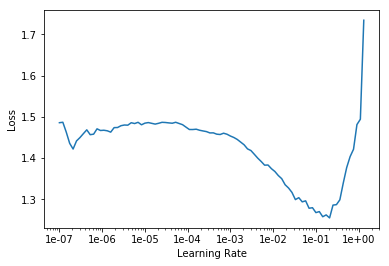
\includegraphics[scale=1]{Figures/clas_lrfinder.png}
\caption{Evolución de la pérdida conforme se cambia la tasa de aprendizaje en el clasificador Al igual que con el LM, se deberá elegir un valor óptimo para mayor eficiencia.}
\label{fig:claslr}
\end{figure}

Primero se eligió un pero para los parámetros de \textit{dropout} y después se eligió un $\gamma$ óptimo (figura \ref{fig:claslr}).

\begin{figure}
\centering
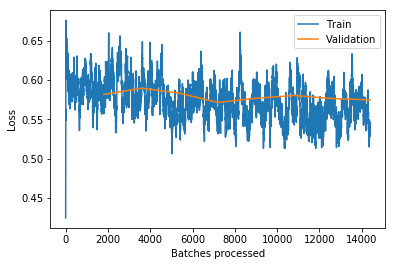
\includegraphics[scale=1]{Figures/clas_epochs.png}
\caption{Avance de pérdida conforme avanzan las épocas de entrenamiento. Menor es mejor.}
\label{fig:clasepochs}
\end{figure}

El entrenamiento de un clasificador con pocos datos no deberá tomar mucho tiempo y los resultados deberán ser satisfactorios aplicando los temas expuestos en este trabajo. En la figura \ref{fig:clasepochs} se puede apreciar como la evolución de pérdida avanza lentamente a través de las épocas y converge en un valor después de un número de épocas relativamente bajo.

\section{Resultados}

Se ha dicho que para RNNs y técnicas de aprendizaje profundo no han tenido el mismo éxito que en otras tareas debido a la dificultad que un modelo de aprendizaje profundo tiene al aprender la cantidad de parámetros inmesa con pocos datos \parencite{zampieri2017, malmasi2016discriminating}. Esta tarea es por lo tanto ideal para poder determinar la capacidad real la transferencia de aprendizaje en NLP y sobre todo cuando las instancias de aprendizaje son limitadas.

Muchos datos de referencia provienen del reporte de la competencia PAN17 \parencite{rangel2017overview} y proveen un contexto para la tarea de perfilamiento. Algunas comparaciones no directas serán realizadas con resultados de la tarea de DSLCC \parencite{zampieri2017}.






